% -----------------------------------------------------------------------------

\begin{frame}{GABA and Glutamate}
    \begin{columns}[c] % The "c" option specifies centered vertical alignment while the "t" option is used for top vertical alignment

        \column{.5\textwidth} % Right column and width
    
        \begin{figure}
        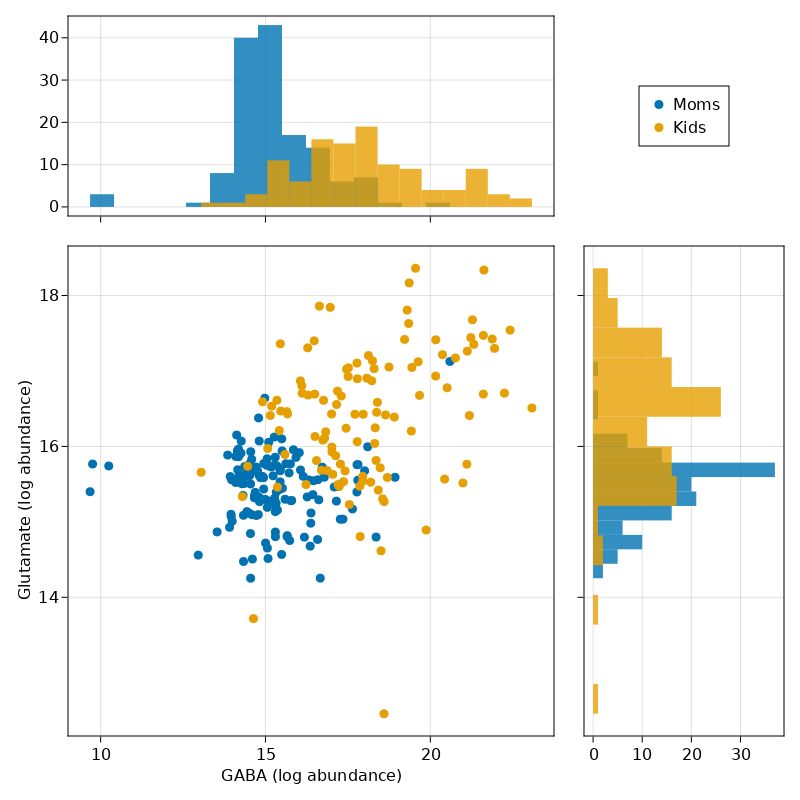
\includegraphics[width=1\linewidth]{../figures/gaba-glutamate.png}
        \end{figure}

        \column{.4\textwidth} % Right column and width
    
        \textbf{Details}
        \begin{enumerate}
            \item Comparing mother and child samples
            \item Mean-centered and compositional
            \item Plotting $log_2(relative\_abundance)$
        \end{enumerate}

    \end{columns}

\end{frame}

% -----------------------------------------------------------------------------

\begin{frame}{GABA and Glutamate, by age}
    \begin{columns}[c] % The "c" option specifies centered vertical alignment while the "t" option is used for top vertical alignment

        \column{.5\textwidth} % Right column and width
    
        \begin{figure}
        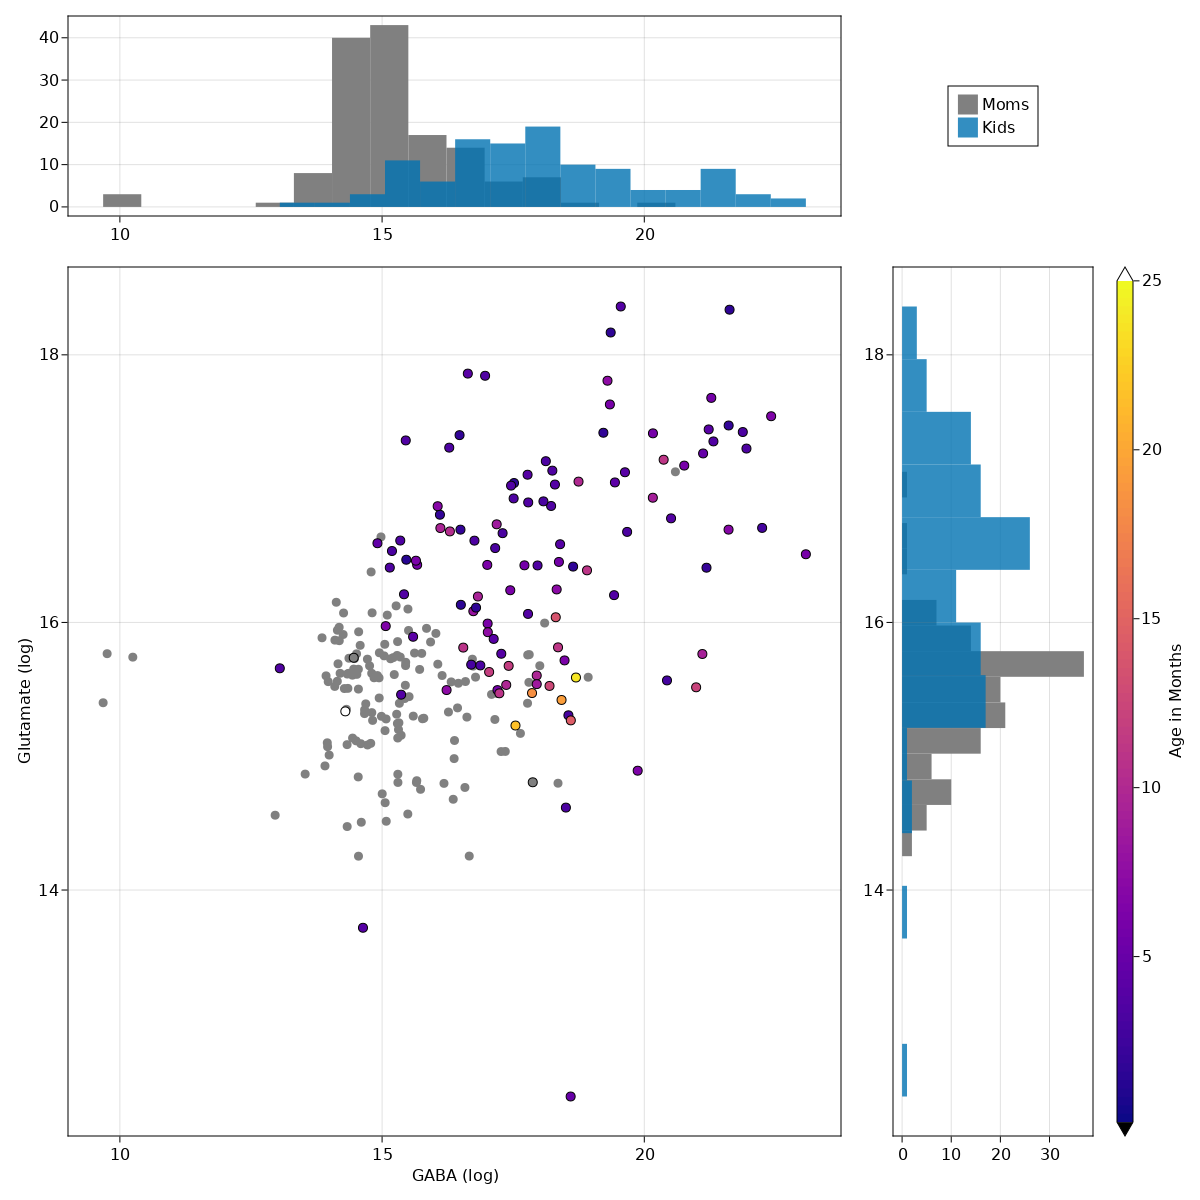
\includegraphics[width=1\linewidth]{../figures/gaba-glutamate_age.png}
        \end{figure}

        \column{.4\textwidth} % Right column and width
    
        \textbf{Details}
        \begin{enumerate}
            \item Comparing mother and child samples
            \item Age in months colored, moms are gray
            \item Plotting $log_2(relative\_abundance)$
        \end{enumerate}

    \end{columns}

\end{frame}

% -----------------------------------------------------------------------------

\begin{frame}{Metabolites PCoA}
    \begin{columns}[c] % The "c" option specifies centered vertical alignment while the "t" option is used for top vertical alignment

        \column{.5\textwidth} % Right column and width
    
        \begin{figure}
        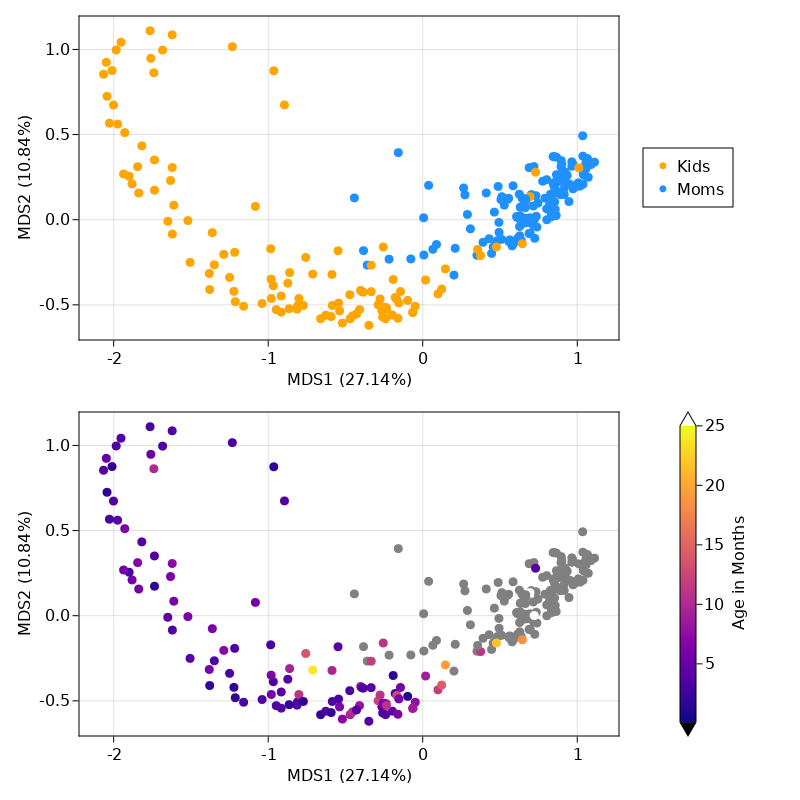
\includegraphics[width=1\linewidth]{../figures/metabolites_pcoa.png}
        \end{figure}

        \column{.4\textwidth} % Right column and width
    
        \textbf{Details}
        \begin{enumerate}
            \item PCoA based on BC dissimilartiy
        \end{enumerate}

    \end{columns}

\end{frame}

% -----------------------------------------------------------------------------
